
\section{Présentation}
Le banc de test correspond au système composé du capteur \gls{capteur} et des appareils des mesures. Pour ce banc de test, le matériel suivant est utilisé :
\begin{itemize}
    \item \textbf{Capteur avec son support (Design 1 ou 5)}\\
          La géométrie générale du Design 1 et 5 est expliquée et représentée au chapitre \ref*{chap:catalogueSol}. \\
          
    \item \textbf{Débitmètre de référence FESTO SFAH-10B-Q6S-PNLK-PNVBA-M8}\\
          Le débitmètre choisi est un débitmètre bidirectionnel avec une entrée d'air de 6 mm de diamètre. Il sera placé juste avant l'entrée du flux
          d'air dans le capteur, permettant ainsi d'avoir une valeur de référence fiable.\\
          
          Un graphe de la tension en fonction du débit fourni par le débitmètre de référence a été construit grâce à la sortie analogique de ce dernier :
          \begin{figure}[H]
              \centering
              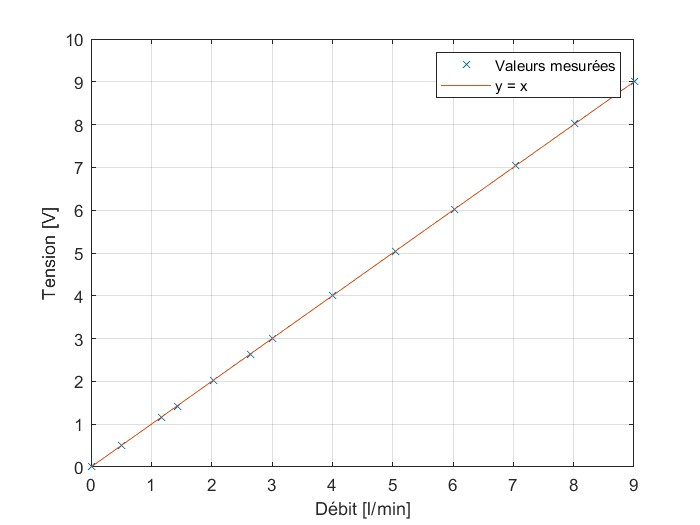
\includegraphics[scale = 0.4]{assets/figures/Calibration_maison.jpg}
              \caption{Tension en fonction du débit}
              \label{fig:calibration}
          \end{figure}
          
          Sur la figure \ref{fig:calibration}, nous pouvons observer la tension mesurée en fonction d'un certain débit d'air. Les paramètres utilisés
          pour cette calibration sont les suivants :
          \begin{itemize}
              \item Sortie analogique en tension sur une plage de 0 V à 10 V
              \item Full Scale allant de 0\% à +100\%
          \end{itemize}
          
          Le graphe montre une fonction linéaire qui se rapproche très fortement de la fonction $y = x$ (f$_{mesur\acute{e}}(x) = 1.0004x - 0.0038$).\\
          
    \item \textbf{Électrovanne FESTO MHE3-MS1H-3/2G-QS-6-K}\\
          Cette électrovanne fonctionne avec une tension de 24 V.  Elle permet de créer un flux d'air pulsé. Ce flux d'air pulsé alimentera le
          capteur \gls{capteur}.\\
          Cet appareil possède 3 ports de connexion et 2 commutations différentes (également dit : vanne à 3/2 voies) disposées selon le schéma ci-dessous :
          \begin{figure}[H]
              \centering
              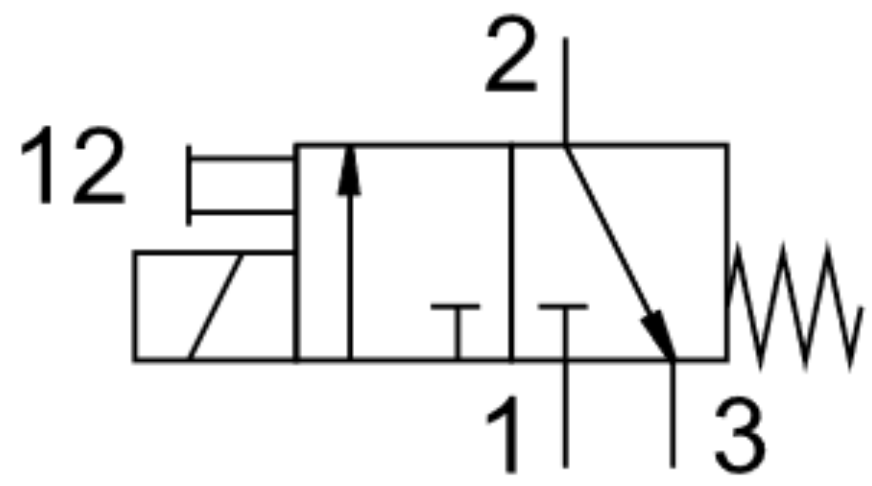
\includegraphics[scale = 0.3]{assets/figures/Electrovanne_InOutput.png}
              \caption{Entrée et sortie de l'électrovanne}
              \label{fig:electrovanne_InOutput}
          \end{figure}
          Les entrées/sorties sont représentées par les numéros 1, 2 et 3. L'électrovanne est représentée par deux carrés accolés (cf. figure
          \ref*{fig:electrovanne_InOutput}). Le carré de gauche montre le système au repos. Le carré de droite représente la deuxième position de
          l'électrovanne, lorsque celle-ci est mise sous tension \cite{mimwebsite}.\\
          
    \item \textbf{Transistor MOSFET IRL540N}\\
          Le MOSFET (metal-oxide-semiconductor field-effect transistor) est un transistor fonctionnant en tension. Dans notre cas, il va
          être utilisé comme un interrupteur qui va alimenter ou non l'électrovanne.
          \begin{figure}[H]
              \centering
              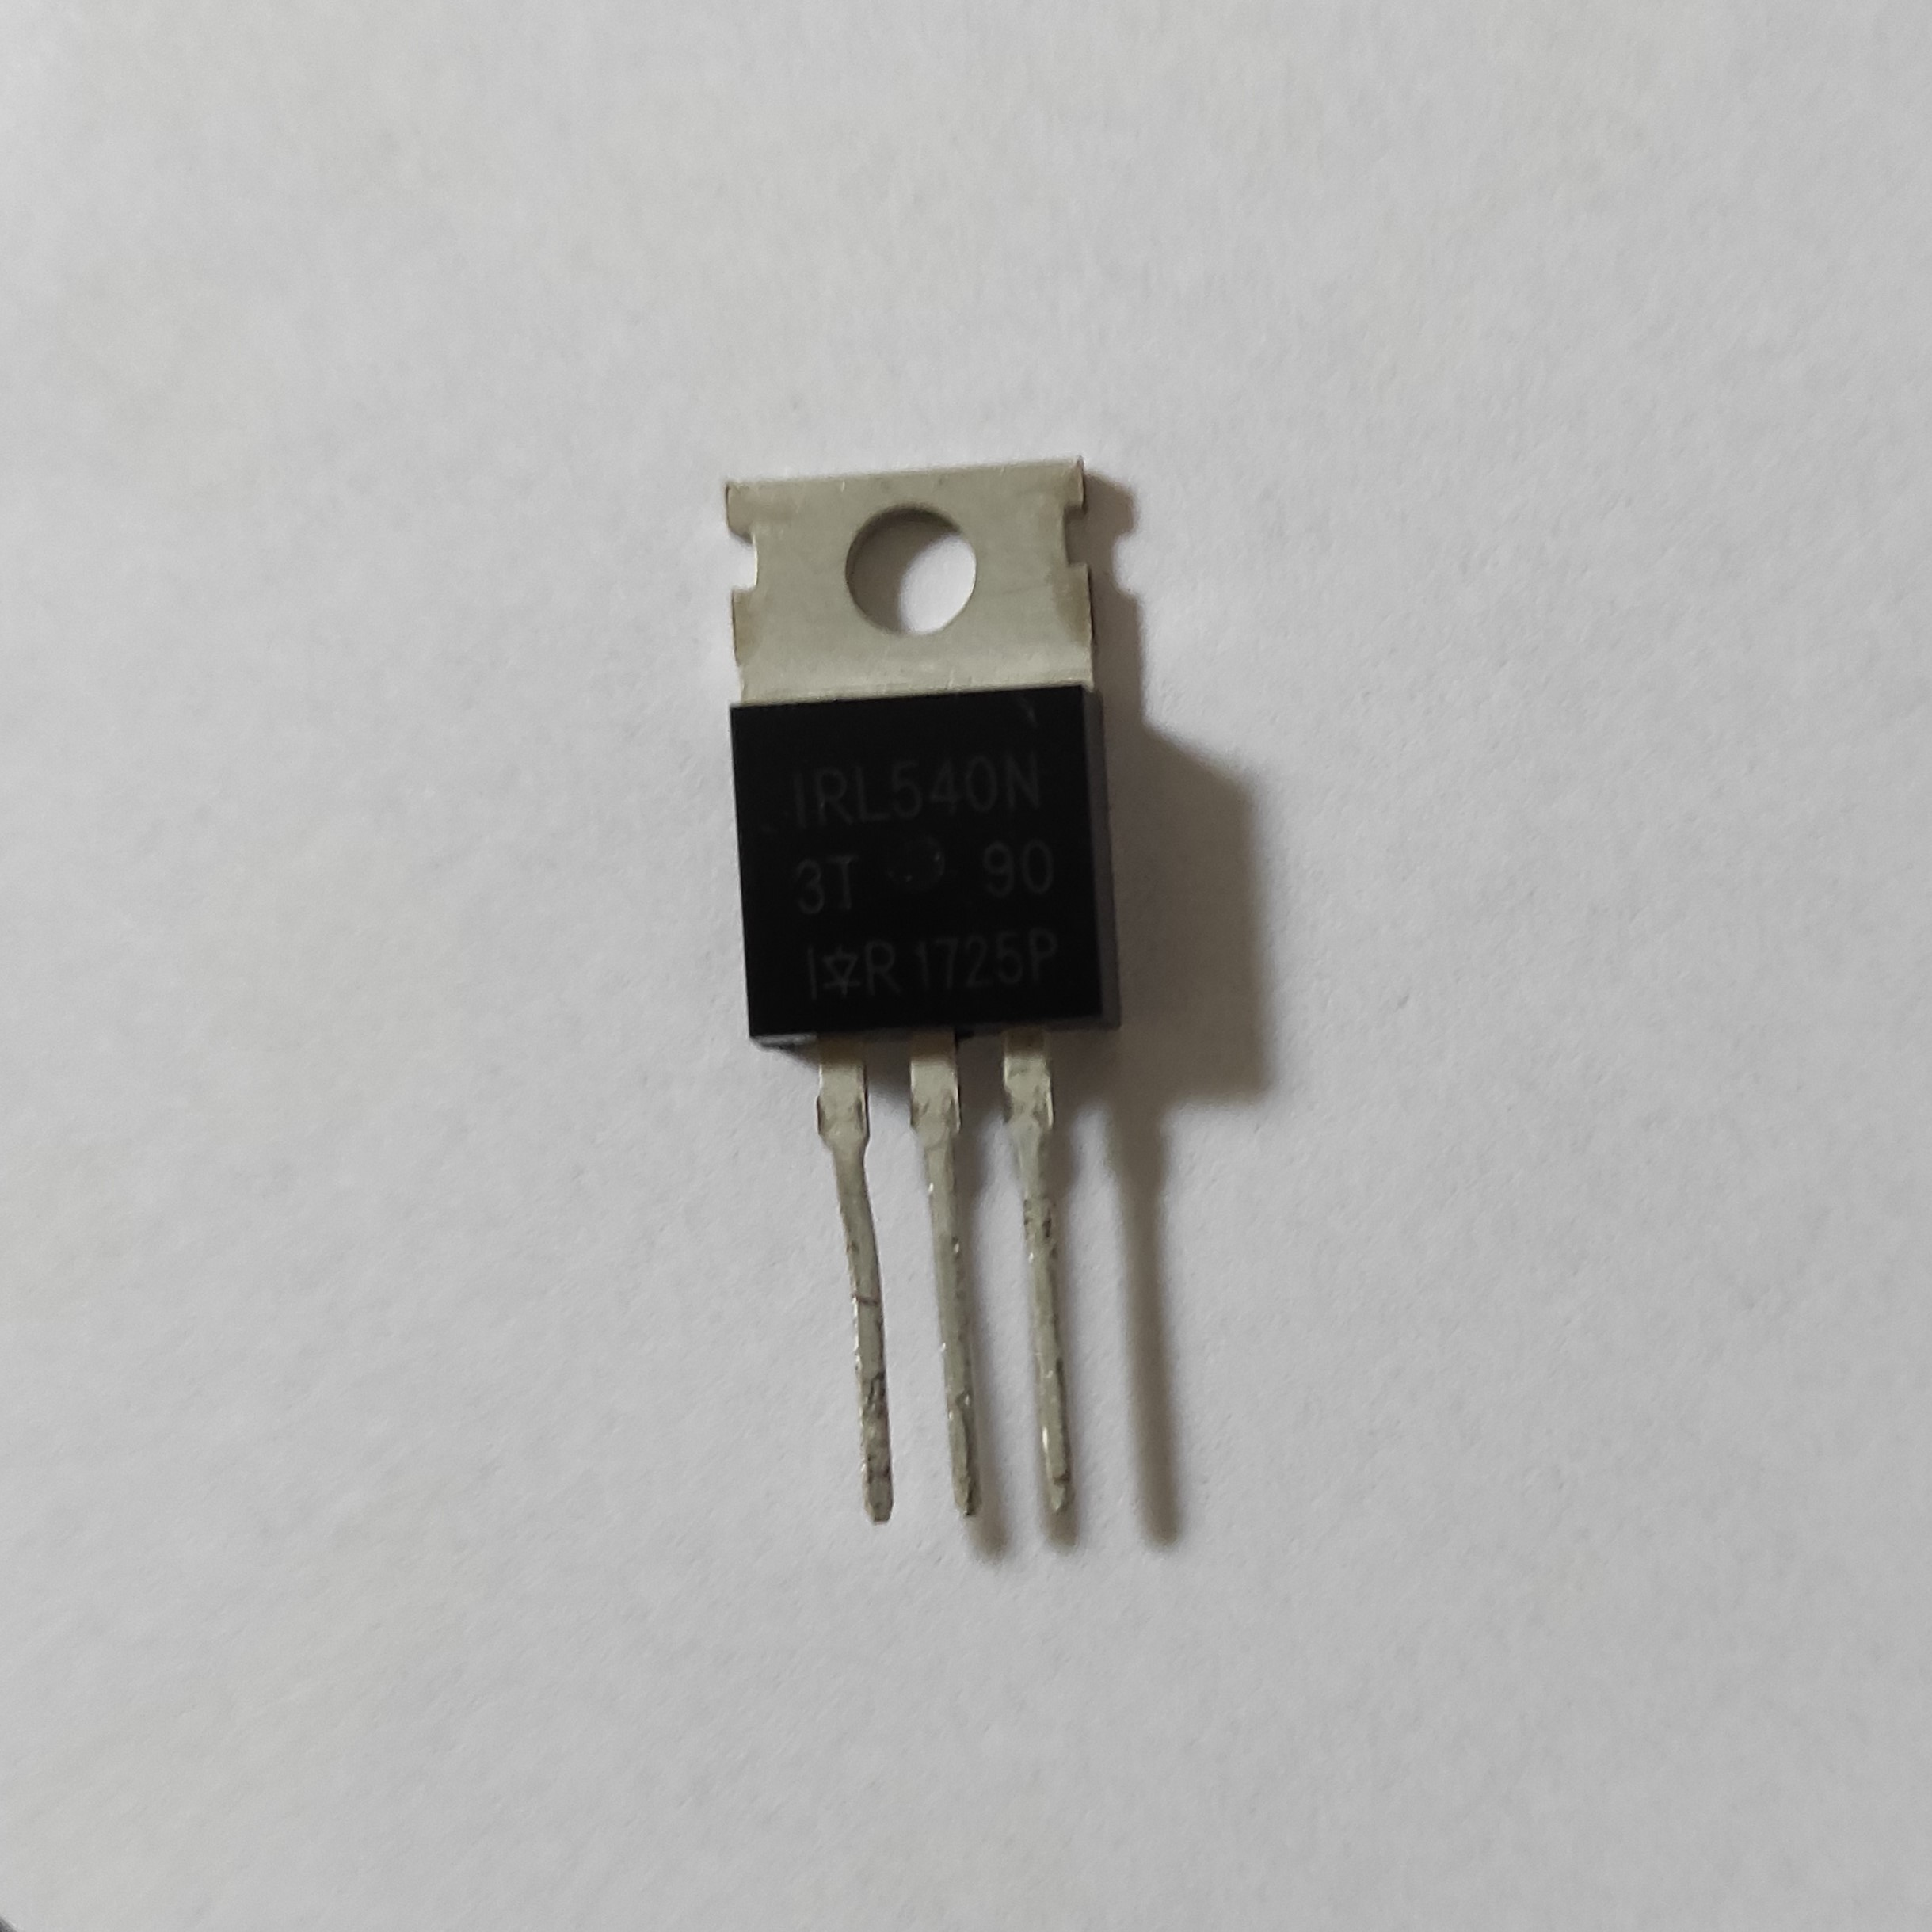
\includegraphics[scale = 0.05]{assets/figures/mosfet_visuel.jpg}
              \caption{MOSFET}
              \label{fig:mosfet}
          \end{figure}
          
    \item \textbf{Arduino Nano}\\
          L'Arduino Nano est un circuit-imprimé qui va également participer à la création du flux d'air pulsé. C'est grâce à l'arduino que la
          fréquence du flux d'air sera modulable. En effet, ce composant va contrôler le MOSFET, qui transmettra ensuite les informations à
          l'électrovanne.\\
          Le code utilisé afin de créer une sortie en tension par pulsation est fourni en annexe. Il a été réalisé sur le logiciel Arduino IDE.\\
          
\end{itemize}

Toutes les Datasheet des composants utilisés et achetés se trouvent en annexe. Ces Datasheet contiennent toutes les valeurs et schéma nécessaire
au dimensionnement du banc de test.

\section{Modélisation du banc de test}
\subsection{Flux d'air pulsé}
Une première solution est d'amener un flux d'air pulsé sur la membrane. Ce flux d'air serait contrôlé par une électrovanne et un
transistor MOSFET IRL540N. Ce transistor a été choisi, car il permet d'être contrôlé grâce à un Arduino Nano. En effet, sa tension de seuil
($V_{GS}$) est de 4 V, 5 V ou 10 V. Étant donné que l'Arduino Nano sortira une tension de 5 V, cette valeur sera suffisante pour faire fonctionner
le MOSFET.
\begin{figure}[H]
    \centering
    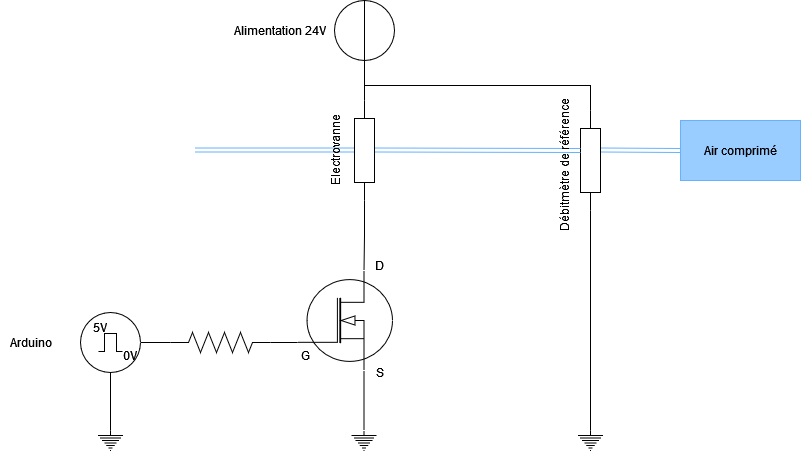
\includegraphics[scale=0.6]{assets/figures/MOSFET.png}
    \caption{Schéma électrique avec MOSFET}
    \label{fig:MOSFET}
\end{figure}
Un contrôle de la chaleur dégagée par effet Joule est utile afin de décider si un dissipateur thermique est nécessaire. Ce calcul se fait
de la manière suivante :\\
D'abord, calculons la chaleur dégagée (puissance par effet Joule) :

\[I_{electrovanne} = \frac{P_{electrovanne}}{U} = \frac{6.5}{24} \cong 0.27 \text{ A} \]
\[P_{effetJoule} = R_{DS}\cdot I^2\]
Avec :\\
$R_{DS}$ (résistance entre les jonctions D et S du MOSFET) = 0.053 $\Omega$

Ainsi :
\begin{equation}
    P_{effetJoule} = 0.053\cdot 0.27^2 \cong 3.86 \text{ mW}
\end{equation}

Les différentes valeurs de résistances, puissances, etc. se trouvent dans la datasheet du MOSFET qui se trouve en annexe. \\

Puis, nous pouvons calculer la puissance maximum dissipée par le MOSFET :
\[P_{max\,dissip\acute{e}e} = \frac{max(T_j) - T_A}{R_{\theta JA}} = \frac{175-25}{62}\cong 2.42 \text{ W}\]
Avec :\\
$T_j$ = température de jonction [\textdegree C]\\
$T_A$ = température ambiante [\textdegree C]\\
$R_{\theta JA}$ = résistance thermique, de jonction à ambiant [$\Omega$]

Ainsi, comme $P_{effetJoule} < P_{max\,dissip\acute{e}e}$, un dissipateur thermique n'est pas nécessaire. \\

Au niveau du fonctionnement général du système, le transistor est commandé par un Arduino Nano qui alimente le MOSFET avec 5 V par pulsation (1 seconde à 5 V et 1 seconde à 0 V). \\
Lorsque le MOSFET reçoit 5V, il s'active et "laisse passer" le courant qui permet à l'électrovanne de s'ouvrir et de faire passer le
flux d'air.
\begin{figure}[H]
    \centering
    \begin{subfigure}[b]{0.45\textwidth}
        \hspace{-1.5cm}
        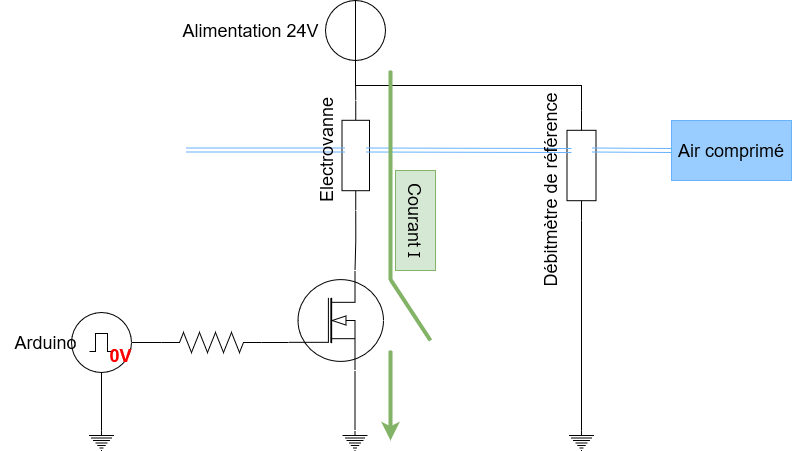
\includegraphics[scale = 0.3]{assets/figures/MOSFET_0V.png}
        \caption{MOSFET non alimenté}
        \label{fig:MOSFET_0V}
    \end{subfigure}
    \begin{subfigure}[b]{0.45\textwidth}
        \centering
        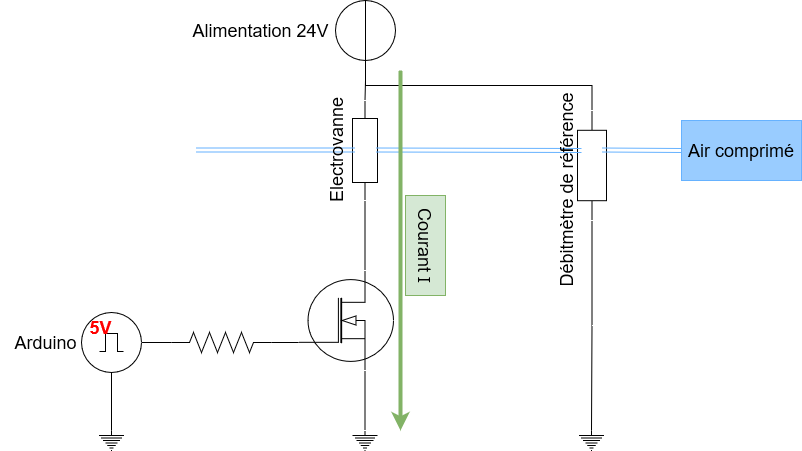
\includegraphics[scale = 0.3]{assets/figures/MOSFET_5V.png}
        \caption{MOSFET alimenté}
        \label{fig:MOSFET_5V}
    \end{subfigure}
    \caption{Fonctionnement du flux d'air pulsé}
    \label{fig:flux_pulse}
\end{figure}

Le corps de chauffe, constitué d'une fine couche d'or, doit être alimenté avec un certain courant. Ce courant, s'il est trop élevé, va abîmer la
membrane, mais s'il est trop bas, il sera insuffisant pour entraîner une différence de température de part et d'autres du capteur. \\

Le calcul suivant a don été effectué afin de déterminer le courant à utiliser pour le corps de chauffe :
\[P_{max} = R\cdot I^2\]
Avec :\\
$P_{parSurface}$ (puissance max par unité de surface) = 100 $\frac{\text{W}}{\text{m}^2}$\\
$R$ (résistance du corps de chauffe) = 45 $\Omega$\\

La valeur de puissance par unité de surface a été tirée de la puissance maximale utilisée pour les chauffages du marché (chauffage au sol).
Elle permet d'avoir un ordre de grandeur pour la valeur de courant à fournir au corps de chauffe.
La surface du corps de chauffe a été approximée à 80 mm$^2$ (2 mm $\cdot$ 40 mm).\\
Ainsi une règle de 3 a été effectuée afin de trouver la valeur de puissance pour le corps de chauffe concerné :
\[P_{max} = 8\cdot 10^{-5}\cdot 100 = 1.78\cdot 10^{-4} \text{ W}\]
\[I = \sqrt{\frac{P_{max}}{R}} = \sqrt{\frac{1.78\cdot 10^{-4}}{45}} \cong 13\text{ mA}\]
Plusieurs tests ont été alors effectué dans une plage de 10 mA à 20 mA. Ces tests ont donné un courant maximum à 15 mA. Au-delà, la membrane
est abîmée (couche d'or rongée).\\

\subsection{Conception 3D et réelle du banc de test}
\begin{figure}[H]
    \centering
    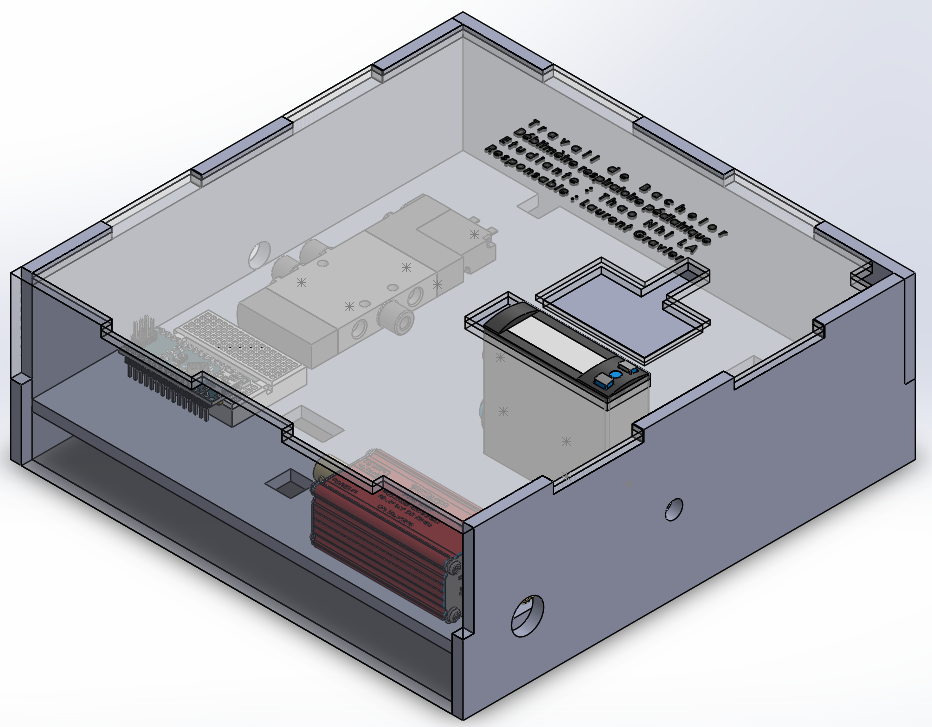
\includegraphics[scale = 0.5]{assets/figures/Banc_de_test.png}
    \caption{Conception 3D du banc de test}
    \label{fig:3D_banc_test}
\end{figure}

\subsection{Corps de chauffe pulsé}
Une autre manière de tester les capteurs \gls{capteur} serait de faire pulser le corps de chauffe et d'amener un flux d'air constant. \\
Cela signifie qu'il faut alimenter le corps de chauffe un certain temps, puis couper l'alimentation. Ceci peut se faire, comme pour l'arrivée
d'air pulsé, par un relais, un transistor tel le MOSFET ou un générateur de fonction. \\

Pour ce projet, un générateur de fonction a été utilisé afin de simplifier le processus. Ce générateur de fonction sortait un signal carré
d'une certaine tension (dépendante de la résistance du corps de chauffe) avec un offset permettant d'avoir un front descendant autour des
0 V. La tension était choisie en fonction de la résistance du corps de chauffe et du courant souhaité (ici 15 mA). En utilisant la loi d'Ohm
$U = R\cdot I$, la tension est facilement calculée.

\section{Vérification du banc de test}
La première version du banc de test est pratique, car lors de la mise en pratique, le flux d'air pulsé est aisément vérifiable. \\
Cependant, lors des premiers tests, aucun signal n'était visible sur l'oscilloscope. Ceci peut être dû à différentes raisons :
\begin{itemize}
    \item Un mauvais contact avec les pointes ressorts\\
          
    \item La puissance du corps de chauffe n'est pas suffisante\\
          
    \item L'échantillon (capteur \gls{capteur}) est défectueux\\
\end{itemize}

Afin de vérifier quel-s paramètre-s entraîne-nt un mauvais résultat, une première décision a été de tester le \gls{capteur} ouvert (sans son support,
en utilisant seulement la membrane).
Des pinces plates viennent faire le contact électrique directement sur les couches d'or afin de mesurer la tension y circulant.
\begin{figure}[H]
    \centering
    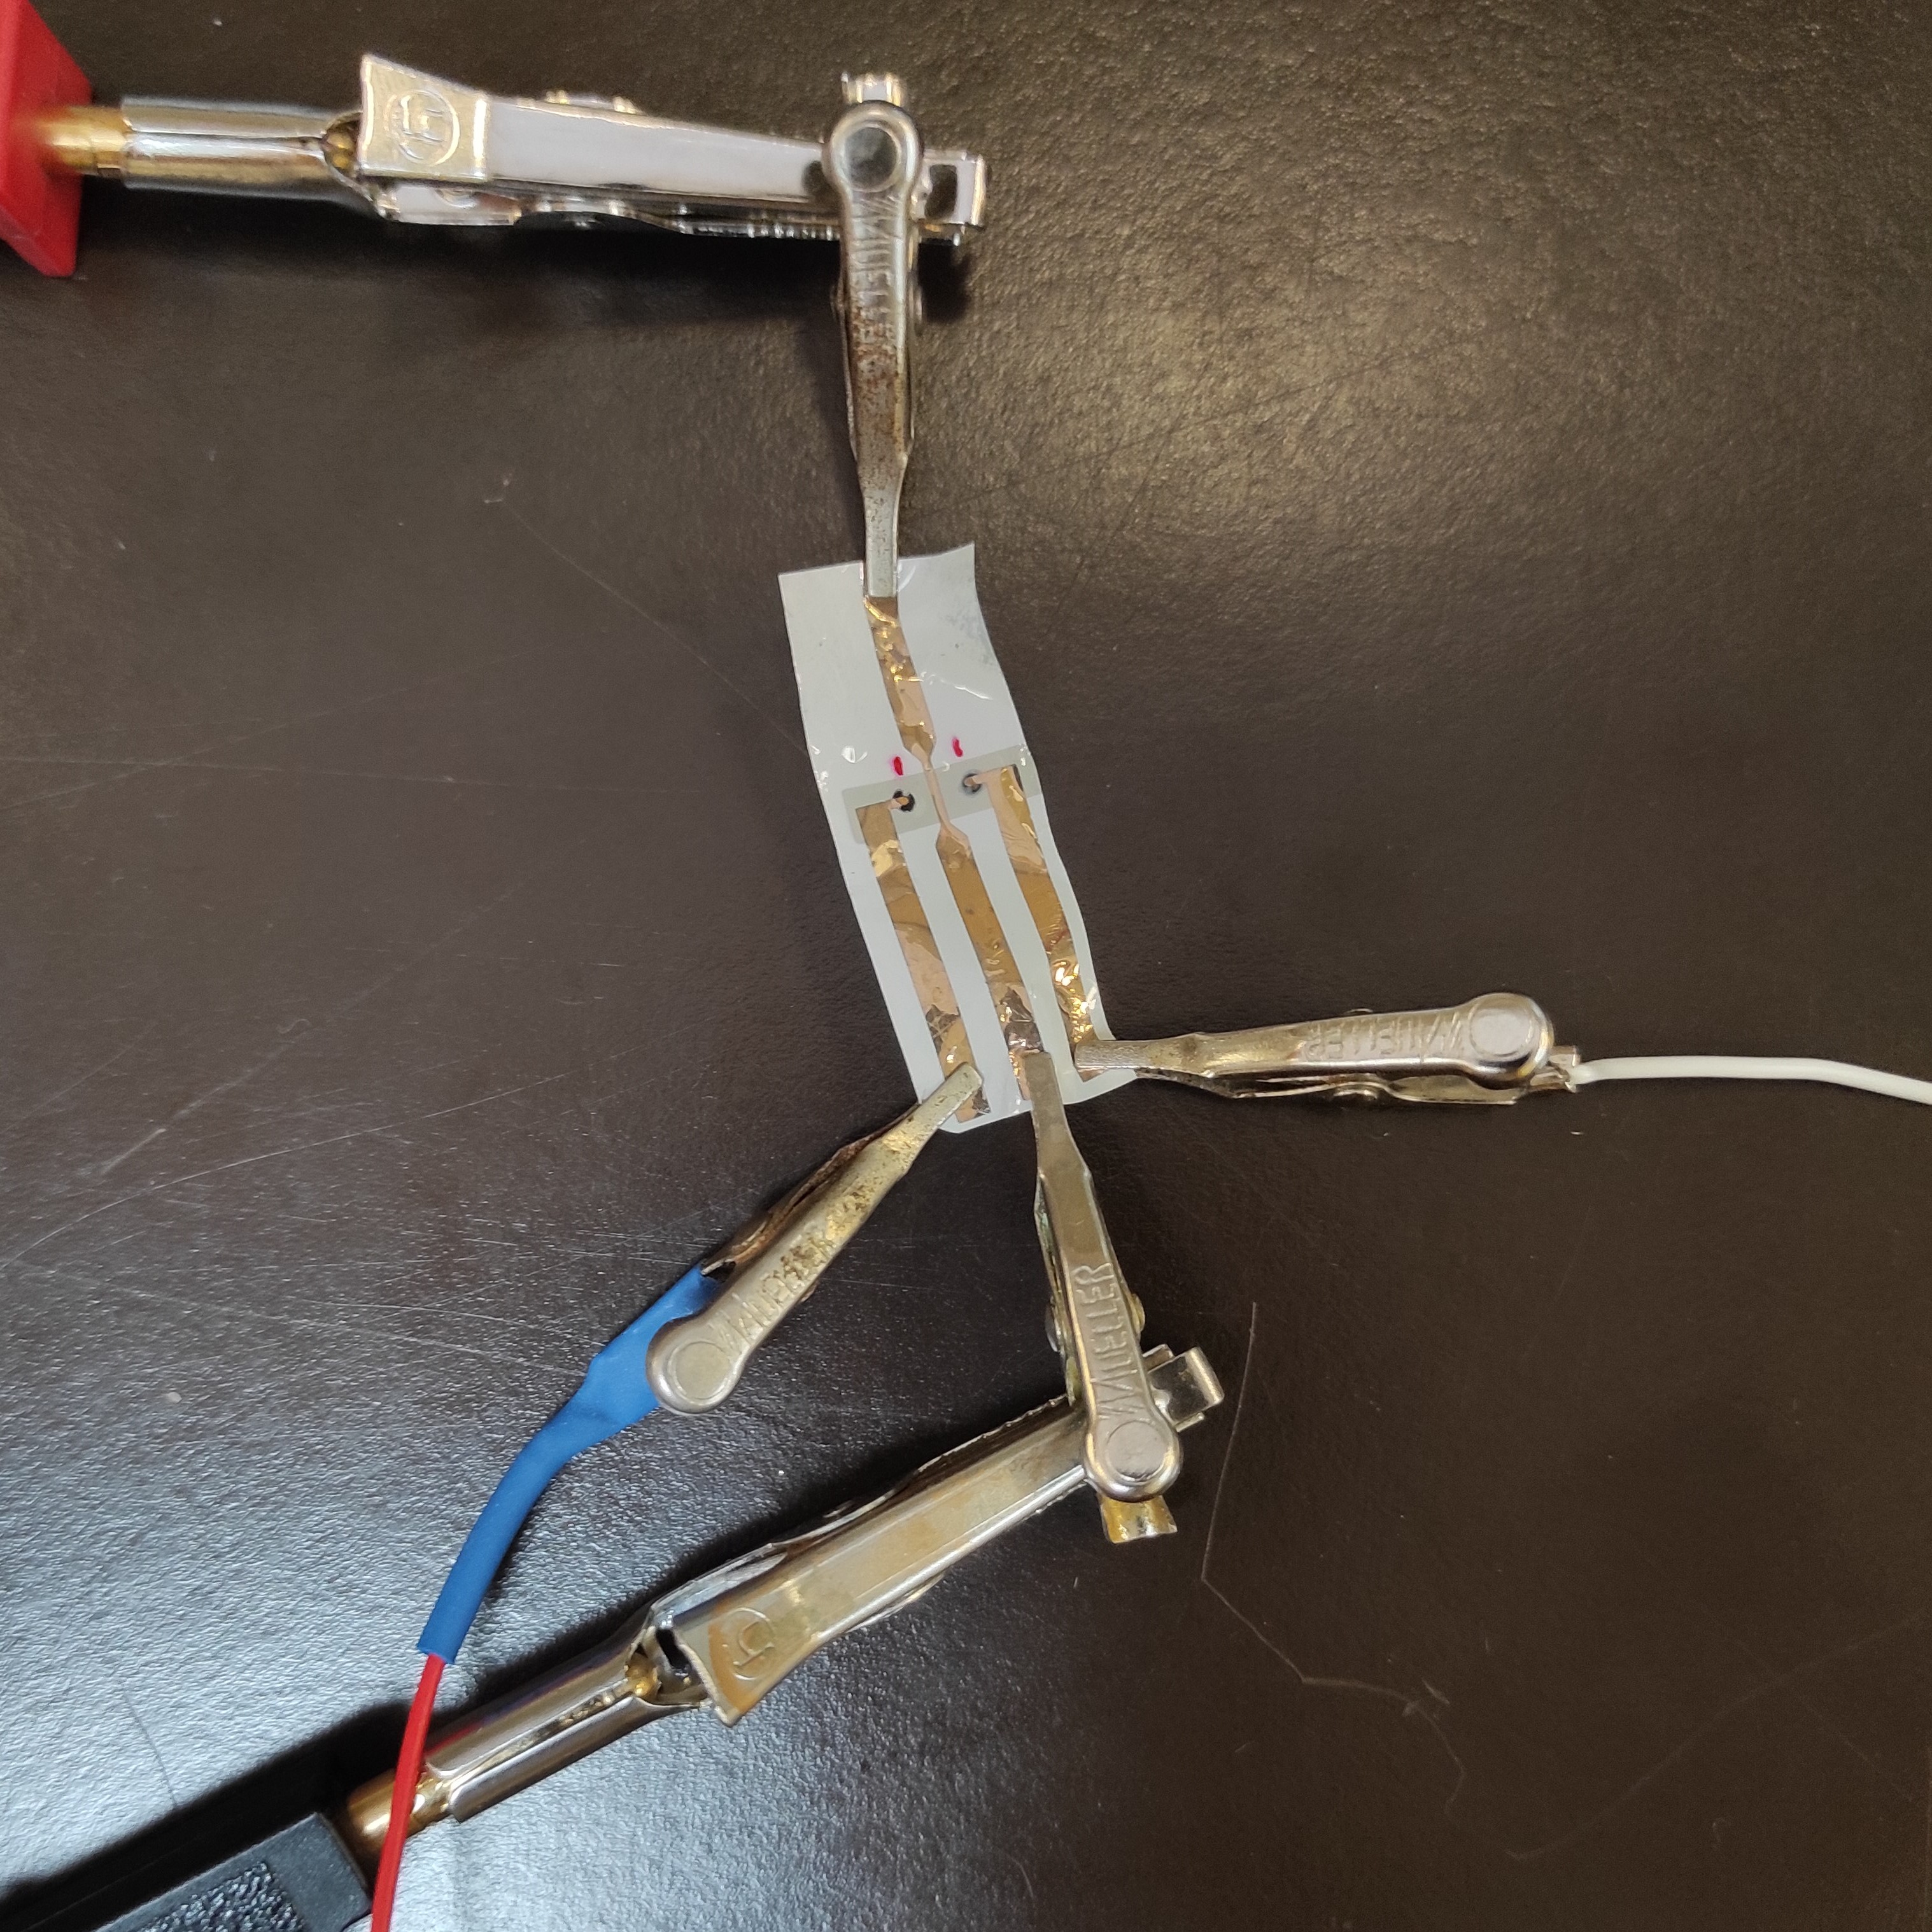
\includegraphics[scale = 0.05]{assets/figures/CapteurOuvert.jpg}
    \caption{Tests sur capteur ouvert}
    \label{fig:capteurOuvert}
\end{figure}
Cette installation ne communiquait pas non plus de résultat concluant (tension oscillant autour des 0 V). \\

Le corps de chauffe a donc été mis en question. Une alternative à ce corps de chauffe a été de venir toucher la pince plate d'un côté du
capteur afin d'engendrer une différence de température entre les deux parties coudées. Ceci a bel et bien entraîné une différence de
température et donc, une tension. Cependant, cette dernière provient de la différence de température entre l'or (sur la membrane) et le métal
de la pince plate. \\

Afin de chauffer une des deux parties électrodéposées, une court tube a été utilisé. Un flux d'air chaud a été soufflé directement sur cette
partie afin de créer un gradient de température, mais à nouveau, aucune fluctuation n'a été perçue. Cependant, lorsque le flux d'air chaud
était soufflé au niveau de la pince plate, une plus grande fluctuation de tension était visible. Cela signifie que la jonction avec le tellure
de bismuth est probablement pathologique.\\

Il était tout de même nécessaire et intéressant de vérifier si le banc de test fonctionnait de manière appropriée. Pour cela, un autre capteur
a été utilisé afin de vérifier la fonctionnalité du banc de test. \\
Le capteur utilisé est un capteur infrarouge par nanotechnologie qui traduit un certain rayonnement électromagnétique en tension. Ainsi lorsque l'on souffle
dessus, un changement dans l'environnement, et plus précisément dans la température ambiante, aura lieu. Ce flux d'air impacte donc
les rayonnements thermiques qui, eux, sont étroitement liés, entre autres, aux rayonnements infrarouges. C'est donc pour cette raison qu'à
l'oscilloscope, une fluctuation sur la tension se dessine.
\begin{figure}[H]
    \centering
    \begin{subfigure}[b]{0.45\textwidth}
        \hspace{-1 cm}
        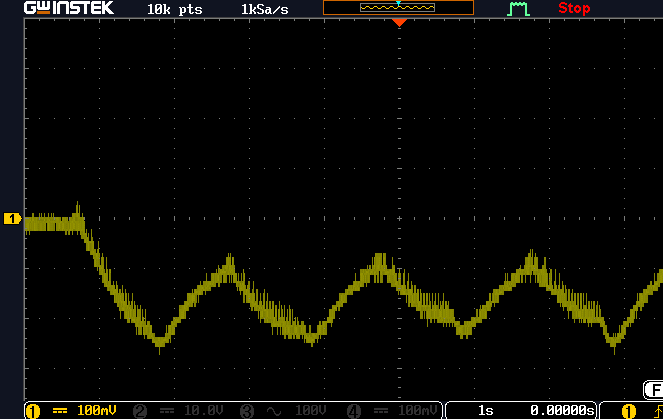
\includegraphics[scale = 0.45]{assets/figures/CapteurIR_1s_1s.PNG}
        \caption{Air pulsé pendant 1 s puis repos pendant 1 s}
        \label{fig:1s1s}
    \end{subfigure}
    \begin{subfigure}[b]{0.45\textwidth}
        \centering
        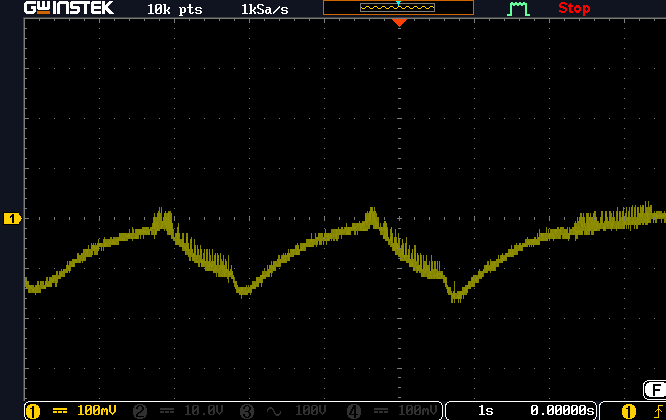
\includegraphics[scale = 0.45]{assets/figures/1_8s_repos.PNG}
        \caption{Air pulsé pendant 1 s puis repos pendant 1.8 s}
        \label{fig:1_8s}
    \end{subfigure}
    \caption{Résultats avec capteur infrarouge}
    \label{fig:capteurIR}
\end{figure}

Les figures ci-dessus (\ref{fig:capteurIR}), montrent que le banc de test et plus précisément, le système de flux d'air pulsé accompagné de
la sortie à l'oscilloscope (en passant par l'amplificateur) fonctionne bien. En effet, sur les figures \ref*{fig:1s1s} et \ref*{fig:1_8s}
les différentes pulsations sont bien visibles.\\

Sur la figure \ref{fig:1s1s}, la récupération du capteur est plus longue que le temps de repos. C'est pourquoi le temps de repos a été allongé
et fixé à 1.8 s (figure \ref*{fig:1_8s}). Ceci permet au capteur de se remettre à zéro et permet aussi de contrôler que la fréquence est bien
modulable. \\

Une autre partie intéressante à étudier est l'amplificateur. Pour ce faire, un petit programme LabView a été utilisé afin de mesurer, dans un
premier temps, la réponse du capteur \gls{infrarouge} sans amplificateur, puis, dans un second temps, la réponse avec amplificateur. Ceci nous
permettra de qualifier l'amplificateur.

Ces tests prouvent que le banc de test semble fonctionner de manière correcte. L'échantillon est alors certainement le facteur engendrant de
mauvais résultats. Un développement de cette thématique sera effectué dans le chapitre \ref{chap:mesures}.

\newpage
\section{Mise en place du banc de test}
\begin{enumerate}
    \item Brancher l'alimentation 24 V au banc de test :
          \begin{itemize}
              \item Connecter le pôle positif de l'alimentation à une des broches de l'électrovanne
              \item Connecter le pôle négatif de l'alimentation à la broche S du MOSFET par le Jumper Wire blanc (il s'agit de la connexion à la terre)
          \end{itemize}
          
    \item Connecter le débitmètre de référence à l'alimentation :
          \begin{itemize}
              \item Connecter le câble marron du débitmètre au pôle positif de l'alimentation (par exemple, grâce à un câble sortant de l'alimentation
                    avec une pince crocodile au bout, lier la broche de l'électrovanne et le fil marron du débitmètre)
              \item Le câble bleu du débitmètre doit être lié à la broche S du MOSFET par le biais du bornier à vis sur la Breadboard
          \end{itemize}
          
          
    \item Brancher le deuxième brin de l'électrovanne à la broche D du MOSFET par le bornier à vis\\
          
    \item Brancher l'amplificateur à une alimentation secteur\\
          
    \item Brancher l'Arduino Nano à un ordinateur et lancer le programme\\
          
    \item Placer le capteur :
          \begin{itemize}
              \item Connecter le corps de chauffe et l'alimentant de maximum 15 mA. Une alimentation de laboratoire peut être utilisée en connectant
                    les deux pointes ressorts concernées par le corps de chauffe à l'alimentation de 15 mA. Les pointes ressorts pour le corps de chauffe
                    sont représentées en jaune sur la figure \ref*{fig:pointes_ressorts_chauffe}.
                    \begin{figure}[H]
                        \centering
                        \begin{subfigure}[b]{0.45\textwidth}
                            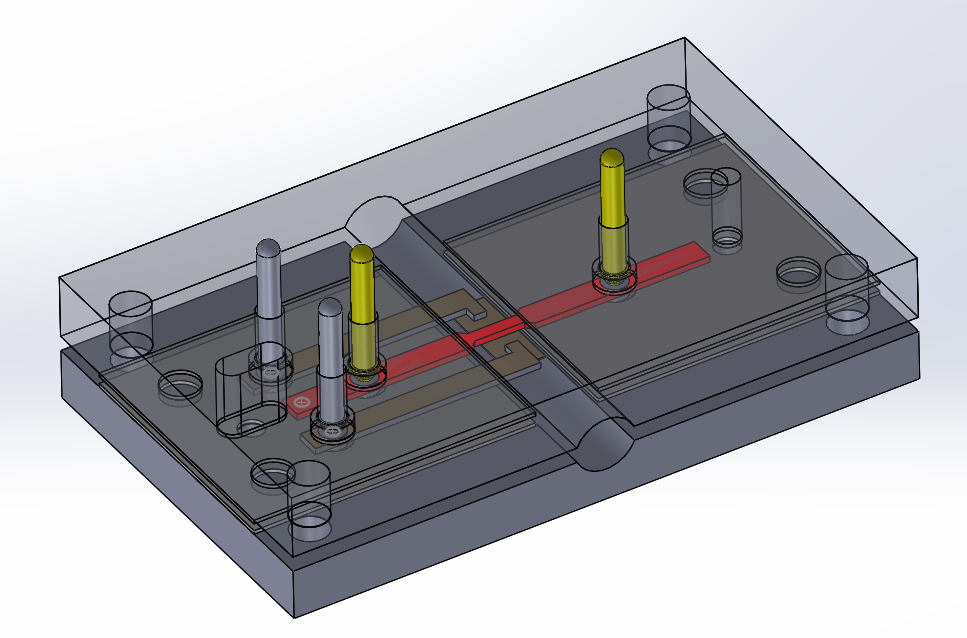
\includegraphics[scale = 0.3]{assets/figures/pointes_ressorts_chauffe.png}
                        \end{subfigure}
                        \begin{subfigure}{0.45\textwidth}
                            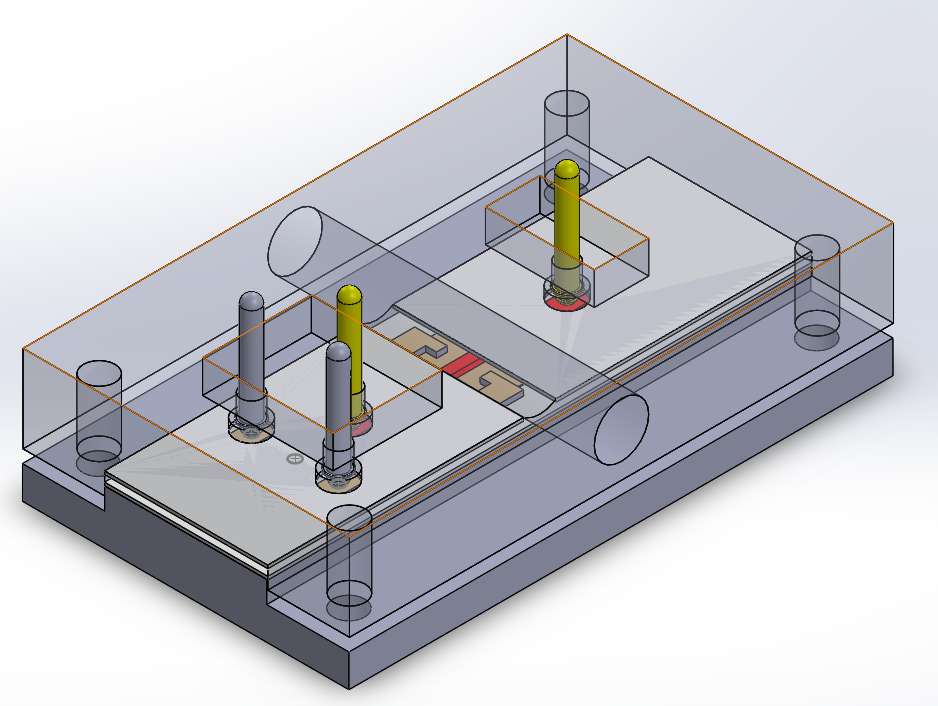
\includegraphics[scale = 0.3]{assets/figures/pointes_ressorts_chauffe_design5.png}
                        \end{subfigure}
                        \caption{Pointes ressorts du corps de chauffe}
                        \label{fig:pointes_ressorts_chauffe}
                    \end{figure}
          \end{itemize}
          
          
    \item Si l'amplificateur est utilisé : Connecter les deux pointes ressorts restantes à l'amplificateur grâce aux câbles sortant en haut
          à droite du banc de test\\
          
    \item Si l'amplificateur n'est pas utilisé : Connecter directement les deux pointes ressorts restantes à l'appareil de mesure utilisé
\end{enumerate}
